\documentclass{minimal}

\usepackage{tikz}
\usetikzlibrary{calc, arrows, fit, positioning, patterns, decorations.pathreplacing}
\tikzstyle{dash} = [dashed, -latex,>=latex]
\tikzstyle{line} = [draw, -latex,>=latex]
\tikzstyle{box} = [draw, minimum size=.8cm]
\tikzstyle{roundbox} = [draw, circle, inner sep=0pt, minimum size=3mm]
\tikzstyle{clamped} = [draw, fill=black, minimum size=0.15cm]

\begin{document}
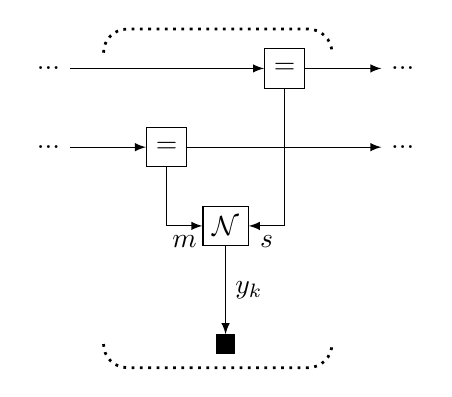
\begin{tikzpicture}
    [
        node distance=15mm,auto,>=latex',
        box/.style={draw, minimum size=.5cm},
        bbox/.style={draw, minimum size=1cm},
        blackbox/.style={draw, fill=black, minimum size=0.25cm}
    ]
    
    \begin{scope}
        %\draw[style=dotted] (0,-10cm) grid[xstep=1cm, ystep=1cm] (12cm,6cm);

        \node[] (s_k_min_1) {$...$};
        \node[box, right of=s_k_min_1, node distance=30mm] (s_eq) {$=$};
        \node[right of=s_eq] (s_k) {$...$};

        \node[below of=s_k_min_1, node distance=10mm] (m_k_min_1) {$...$};
        \node[box, right of=m_k_min_1] (m_eq) {$=$};
        \node[below of=s_k, node distance=10mm] (m_k) {$...$};

        \node[box] (g) at (2.25, -2.0) {$\mathcal{N}$};        
        \node[clamped, below of = g] (y) {};

        \draw[line] (s_eq) -- ($(s_eq)+(0,-2.0)$) -> node[anchor=north]{$s$} (g);
        \draw[line] (m_eq) -- ($(m_eq)+(0,-1.0)$) -> node[anchor=north]{$m$} (g);

        \path[line] (g) edge[->] node[anchor=west]{$y_k$} (y);

        \path[line] (s_k_min_1) -> (s_eq);
        \path[line] (s_eq) -> (s_k);
        \path[line] (m_k_min_1) -> (m_eq);
        \path[line] (m_eq) -> (m_k);

        \draw[dotted, rounded corners=0.3cm, line width = 1pt] ($(1.0,0.2)+(-0.3,0)$) -- ($(1.0,0.2)+(-0.3,0.3)$) -- ($(3.3,0.2)+(0.3,0.3)$) -- ($(3.3,0.2)+(0.3,0)$);
        \draw[dotted, rounded corners=0.3cm, line width = 1pt] ($(1.0,-3.5)+(-0.3,0)$) -- ($(1.0,-3.5)+(-0.3,-0.3)$) -- ($(3.3,-3.5)+(0.3,-0.3)$) -- ($(3.3,-3.5)+(0.3,0)$);
    \end{scope}    

\end{tikzpicture}
\end{document}